\section{Introduction} 
Semantic parsing is used as a component for natural language understanding in human-robot interaction systems \cite{lauria2001training, bos2007spoken, tellex2011understanding, matuszek2013learning, thomason2019improving}, and for virtual assistants  \cite{campagna2017almond, kollar2018alexa, campagna2019genie}.  We would like to be able to apply deep learning methods in this space, as recently researchers have shown success with these methods for semantic parsing more generally, e.g. \cite{dong2016language, jia2016data, zhong2017seq2sql}. However, to fully utilize powerful neural network approaches, it is necessary to have large numbers of training examples. In the space of human-robot (or human-assistant) interaction, the publicly available semantic parsing datasets are small. Furthermore, it can be difficult to reproduce the end-to-end results (from utterance to action in the environment) because of the wide variety of robot setups and proprietary nature of personal assistants.

In this work, we introduce a new semantic parsing dataset for human-bot interactions. Our ``robot'' or ``assistant''  is embodied in the sandbox construction game Minecraft\footnote{\url{https://minecraft.net/en-us/}.  We limit ourselves to creative mode for this work}, a popular multiplayer open-world voxel-based crafting game. We also provide the associated platform for executing the logical forms in game.

Situating the assistant in Minecraft has several benefits for studying task oriented natural language understanding (NLU). Compared to physical robots, Minecraft allows less technical overhead irrelevant to NLU, such as difficulties with hardware and large scale data collection. On the other hand, our bot has all the basic in-game capabilities of a player, including movement and placing or removing voxels. Thus Minecraft preserves many of the NLU elements of physical robots, such as discussions of navigation and spatial object reference. 
 
%\begin{figure*}[t!]
%    \centering
%%     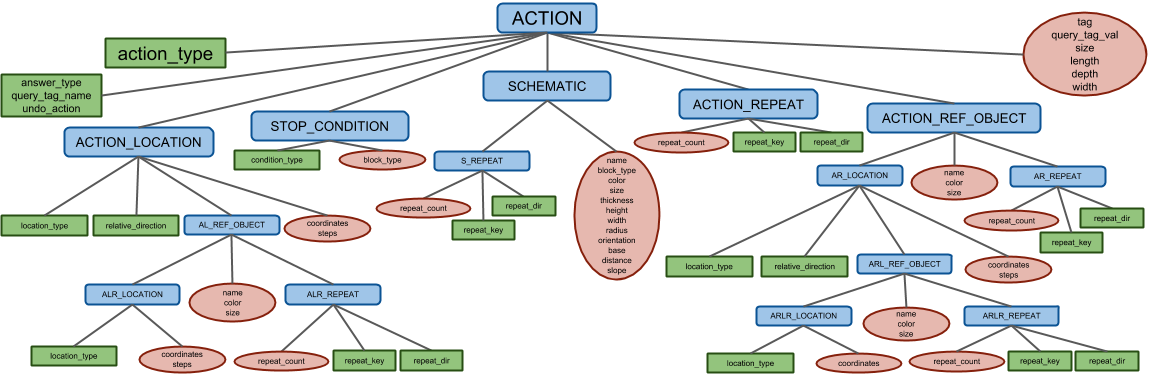
\includegraphics[natwidth=\linewidth]{figures/ActionGrammar.png}
%    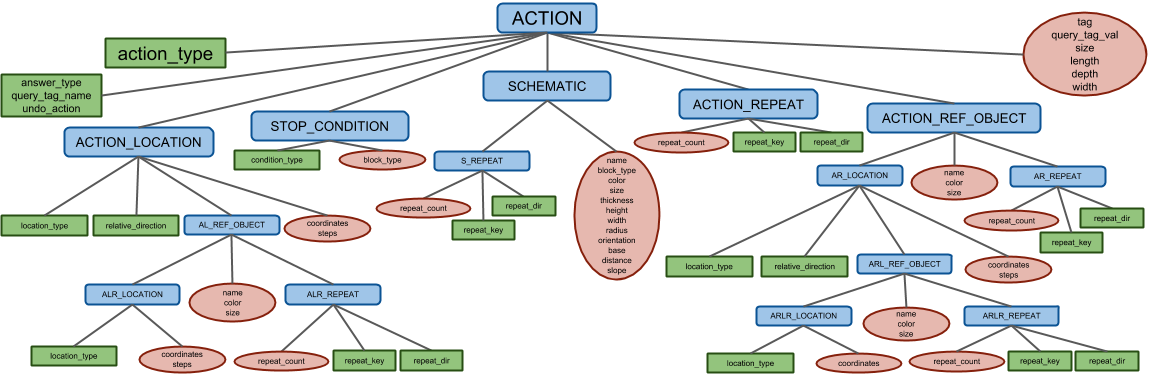
\includegraphics[width=\linewidth]{figures/ActionGrammar.png}
%    \caption{Action space grammar}
%    \label{fig:action_grammar}
%\end{figure*}  


Working in Minecraft may enable large scale human interaction because of its large player base, in the tens of millions. 
 %Compared with personal assistants, Minecraft offers a low
% for allows the possibility of interacting with large number of players
Furthermore, although Minecraft's simulation of physics is simplified, the task space is complex. 
While there are many atomic objects in the game, such as animals and block-types, that require no perceptual modeling, the player also interacts with complex structures made up of collections of voxels such as a ``house'' or a ``hill''. The assistant cannot apprehend them without a perceptual system, creating an ideal test bed for researchers interested in the interactions between perception and language. 

Our contributions in the paper are as follows:
\newline
\noindent{\bf Grammar:} We develop a grammar over a set of primitives that comprise a mid-level interface to Minecraft for machine learning agents.  %See Section \ref{sec:grammar}.
\newline 
\noindent{\bf Data:} %Using a collection of templates to convert logical forms over the primitives into pseudo-natural language, we build a dataset of language instructions with logical form annotation.
% by having crowd-sourced workers rephrase the language outputs, as in \cite{wang2015building}.  
We collect ~7K  crowd-sourced annotations of commands generated independent of our grammar. %, see Section \ref{sec:data}. 
In addition to the natural language commands and the associated logical forms, we release the tools used to collect these, which allow crowd-workers to efficiently and accurately annotate parses.%; see Section \ref{sec:annotation}.
%We hope in addition to use as a semantic parsing dataset, these will be useful for researchers in reinforcement learning.
\newline   
\noindent{\bf Models:} We show the results of several neural semantic parsing models trained on our data. %See Section \ref{sec:modeling} and \ref{sec:experiments}.
\newline   
\noindent{\bf Execution:} Finally, we also make available the code to execute logical forms in the game, allowing the reproduction of end-to-end results.  This also opens the door to using the data for reinforcement and imitation learning with language.
We also provide access to an interactive bot using these models for parsing\footnote{Instructions can be found at \url{http://craftassist.io/acl2020demo}, requires a Minecraft license and client.}. %We demonstrate  that adapting the neural architecture to the grammar can improve parsing accuracy.

%\begin{figure*}[t!]
 %   \centering
%%    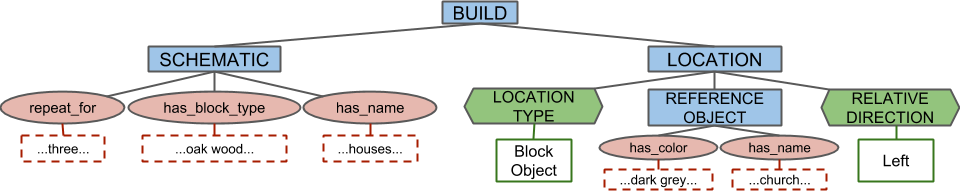
\includegraphics[natwidth=\linewidth ]{figures/ExampleParse.png}
 %   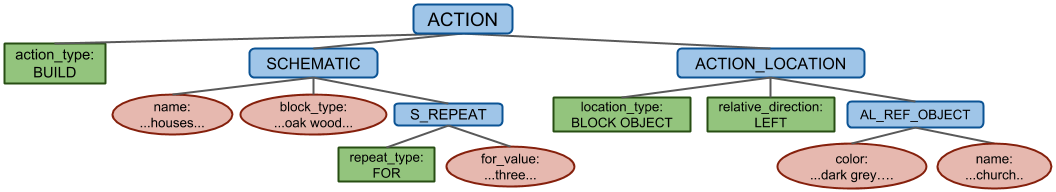
\includegraphics[width=\linewidth ]{figures/ExampleParseNew.png}
 %   \caption{Parse tree for ``Make three oak wood houses to the left of the dark grey church.''    \label{fig:example_parse}
%}
%\end{figure*}


%Advantages of working with MC / game environment -- General usefulness of a large semantic parsing dataset in the context of a semi-tractable virtual environment.

